\chapter{Badania eksperymentalne}
\section{Organizacja eksperymentów}
W poniższym rozdziale wybrane modele z rozdziału \ref{chap:ChangeDetectionAlgo} zostaną,
w celu zbadania efektywności algorytmów,
przetestowane na losowych zbiorach danych.
Platforma na której uruchomiono wszystkie testy to Apache Storm.
Sekcja ta została podzielona na dwie części.
Pierwsza przedstawia szczegółową analizę problemu z wykorzystaniem badanych metod,
natomiast w części drugiej znajdują się zbiorcze wyniki przeprowadzonych doświadczeń.

Analizie eksperymentalnej zostaną poddane algorytmy:
\begin{itemize}
  \item Bayesa,
  \item ADWIN z testem opartym o średnią,
  \item ADWIN z testem opartym o stosunek gęstości rozkładu.
\end{itemize}

W badaniach będą wykorzystane zbiory danych wygenerowane losowo jak i rzeczywiste,
pochodzące z prawdziwych czujników.
\subsection*{Dane wygenerowane losowo}
Dla każdego z testów wygenerowano 20 zbiorów danych.
Każdy ze zbiorów liczył 5000 elementów.
Zmiana wprowadzana była co 100 próbek.
Jako poprawnie wykrytą zmianę uważano zmianę otrzymaną za pomocą algorytmu,
która była w odległości $\pm$ 20 próbek od prawdziwego punktu zmiany.

\subsubsection*{Skacząca średnia}
Jednowymiarowy model auto-regresji wykorzystany przez Liu (Liu i in., 2013)
zostanie użyty do wygenerowania 5000 próbek.
Wartości są opisane wzorem:
$$y(t) = 0.6y(t-1) - 0.5y(t-2) + \varepsilon_t,$$
gdzie $\varepsilon_t$ jest szumem opisanych rozkładem Gaussa z średnią $\mu$
i odchyleniem standardowym równym 1,5.
Zmianie co 100 próbek ulegała średnia szumu $\mu$.
\[ \mu_N =
  \begin{cases}
    0       & \quad N = 1\\
    \mu_{N-1} + \frac{N}{16} & \quad N = 2,3, \ldots, \\
  \end{cases}
\]
gdzie N to liczba naturalna równa indeksowi aktualnej zmiany.
\subsubsection*{Rozkład dwuwymiarowy -- zamiana kowariancji}
Do badania użyto 5000 próbek pobranych z dwuwymiarowego rozkładu normalnego.
Zmiana występuje co 100 próbek
i polega na modyfikacji macierzy kowariancji $\Sigma$.
\[ \Sigma =
  \begin{cases}
    \begin{pmatrix} 1 & -\frac{4}{5} - \frac{N-2}{500} \\ -\frac{4}{5} - \frac{N-2}{500} & 1 \end{pmatrix} & \quad N = 1,3,\ldots\\
    \begin{pmatrix} 1 & \frac{4}{5} + \frac{N-2}{500} \\ \frac{4}{5} + \frac{N-2}{500} & 1 \end{pmatrix} & \quad N = 2,4,\ldots\\
  \end{cases}
\]
\subsubsection*{Badanie sprawności}
Do oceny sprawności algorytmów wykorzystano miary zapraponowane przez Liu (Liu i in., 2013):
\begin{itemize}
  \item współczynnik sukcesów (\textit{true positive rate, TPR}): $n_{s}/n_{c}$,
  \item współczynnik fałszywych alarmów (\textit{false positive rate, NPR}): $(n_{a}-n_{s})/n_{a}$,
\end{itemize}
gdzie $n_{s}$ to liczba poprawnie wykrytych zmian, $n_{c}$ to liczba wprowadzonych zmian,
a $n_{a}$ to liczba wszystkich wykrytych zmian.

\subsection*{Dane rzeczywiste}
Dane rzeczywiste zebrano za pomocą czujnika światła oraz czujnika zbliżeniowego.
Czujniki leżały na biurku i skierowane pionowo w kierunku sufitu.
Przykładowe wyniki czujników przedstawiono w tabeli \ref{tab:DeviceValues}.
Wykres \ref{fig:DeviceValues} przedstawia przebiegi ostatnich 5000 próbek.
Dane zostały przekazane przez opiekuna naukowego pracy dr inż. Janusza Granata.
\subsubsection*{Czujnik światła}
Czujnik mierzył natężenie światła w otoczeniu.
Na wartości wpływ ma nie tylko fakt przesłonięcia go przez przedmiot,
ale także pora dnia.
\subsubsection*{Czujnik odległości}
Czujnik zbliżeniowy mierzy odległość od najbliższego przedmiotu,
wynik był podawany w cm.
\begin{table}[h]
  \label{tab:DeviceValues}
  \centering
  \begin{tabular}{r r}
    \multicolumn{1}{l}{Odległość} & \multicolumn{1}{l}{Natężenie} \\
    \hline
    266.34 & 0566 \\
    266.34 & 0567 \\
    266.32 & 0566 \\
    266.77 & 0566 \\
    266.84 & 0567 \\
    266.36 & 0567 \\
    266.73 & 0568 \\
    266.29 & 0566 \\
    266.68 & 0565 \\
    266.29 & 0566 \\
    266.36 & 0566 \\
    266.32 & 0567 \\
    266.72 & 0568 \\
    266.77 & 0567 \\
  \end{tabular}
  \caption{Wartości czujników}
\end{table}
\begin{figure}[htbp]
  \centering
  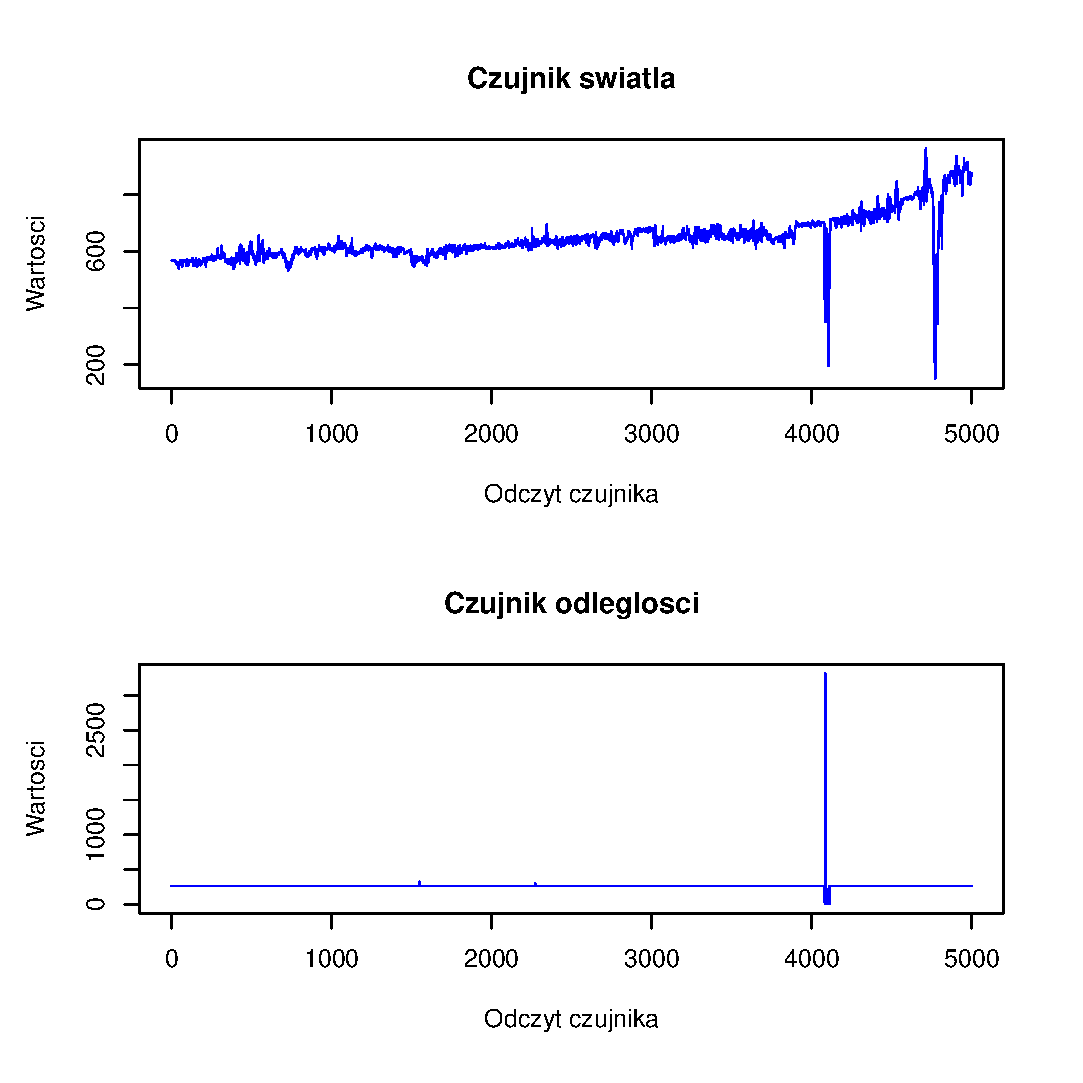
\includegraphics[width=1\textwidth]{img/ch-5-device}
  \caption{Wartości czujników}
  \label{fig:DeviceValues}
\end{figure}
\newpage
\section{Wyniki eksperymentów}
W poniższym rozdziale zostaną przedstawione wyniki przeprowadzonych badań.
Dla poprawy czytelności przyjęto następujące oznaczenia:
\begin{itemize}
  \item algorytm Bayesa oznaczono BAY,
  \item algorytm ADWIN z testem na średnią oznaczono $ADW_{\mu}$,
  \item algorytm ADWIN z testem na gęstość oznaczono $ADW_{d}$
\end{itemize}

\subsection{Skacząca średnia}
Na wykresie \ref{fig:JumpingValues} przedstawiono przykładowy przebieg wartości dla pierwszych 5 zmian
wraz z zaznaczonymi miejscami,
gdzie nastąpiła.
\begin{figure}[htbp]
  \centering
  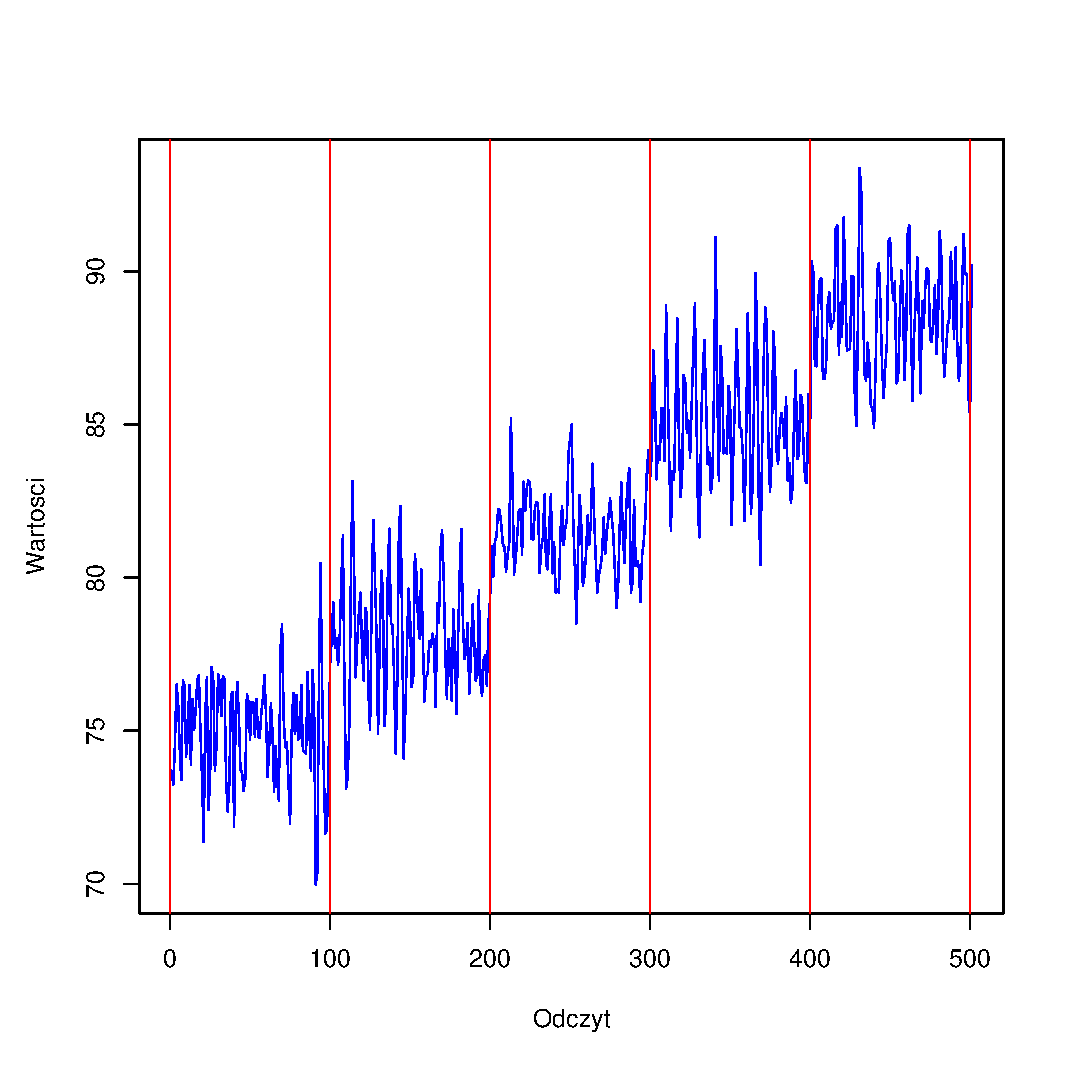
\includegraphics[width=0.5\textwidth]{img/ch-5-jumping}
  \caption{Przykładowe wartości}
  \label{fig:JumpingValues}
\end{figure}
Badanie przeprowadzono poprzez wygenerowanie 20 zestawów danych.
Źródło (\textit{seed}) dla każdego z zestawów były inne.

Na wykresach \ref{fig:JumpingValuesResTpr} i \ref{fig:JumpingValuesResNpr} przedstawion otrzymane wyniki.
Na osi OX zaznaczono kolejne przeprowadzone próby.
Na osi OY przedstawiono odpowiednio współczynnik suksesów (TPR) i fałszywe alarmy (NPR).
Jeśli chodzi o skuteczność (TPR) widać wyraźną przewagę algorytmów z rodziny ADWIN.
Praktycznie w każdej z prób częsciej wykrywały zajście zmiany.
Różnice pomiędzy $ADWIN_d$,
a $ADWIN_{\mu}$ są niezauważalne i z powodzeniem można korzystać z obu.
Niestety jeśli chodzi generowanie fałszywych alarmów wszystkie badane algorytmy
mają zbliżony do siebie poziom.

Zbiorcze wyniki testów przedstawono w tabeli \ref{tab:JumpingResult}.
\begin{table}[h]
  \label{tab:JumpingResult}
  \centering
  \begin{tabular}{l r r r r}
    & \multicolumn{2}{l}{TPR} & \multicolumn{2}{l}{NPR} \\
    \hline
    & \multicolumn{1}{l}{Średnia} & \multicolumn{1}{l}{Wariancja}& \multicolumn{1}{l}{Średnia} & \multicolumn{1}{l}{Wariancja} \\
    \hline
    BAY & 0,439 & $0,887 \times 10^{-3}$ & 0,689 & $1,213 \times 10^{-3}$  \\
    $ADW_{\mu}$ & 0,526 & $1,246 \times 10^{-3}$ & 0,727 & $1,539 \times 10^{-3}$ \\
    $ADW_{d}$ & 0,516 & $2,508 \times 10^{-3}$ & 0,712 & $2,627 \times 10^{-3}$ \\
  \end{tabular}
  \caption{Zbiorcze wyniki testów}
\end{table}

\begin{figure}[htbp]
  \centering
  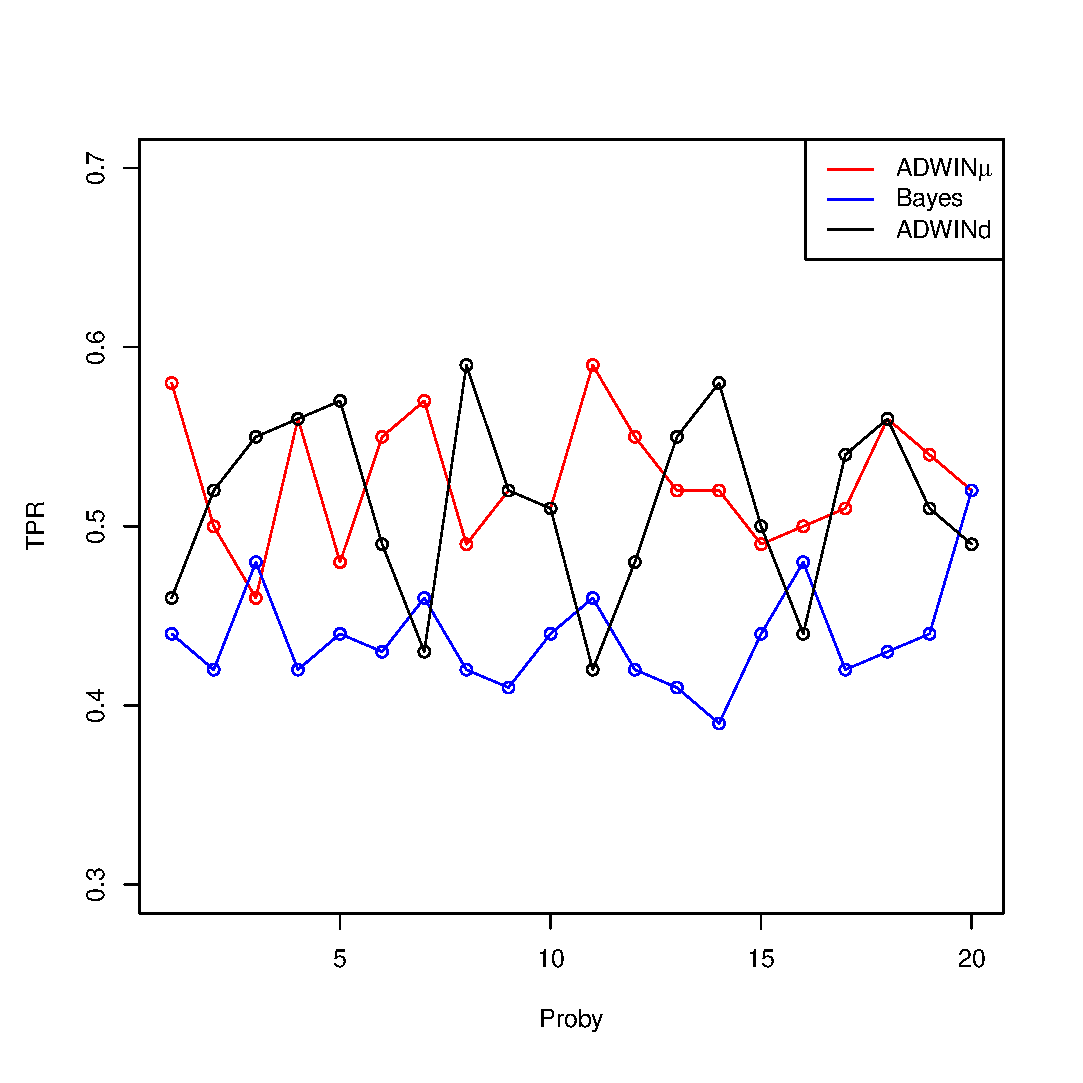
\includegraphics[width=0.6\textwidth]{img/ch-5-jump-res-tpr}
  \caption{Wyniki dla poszczególnych prób -- współczynnik suksesów}
  \label{fig:JumpingValuesResTpr}
\end{figure}
\begin{figure}[htbp]
  \centering
  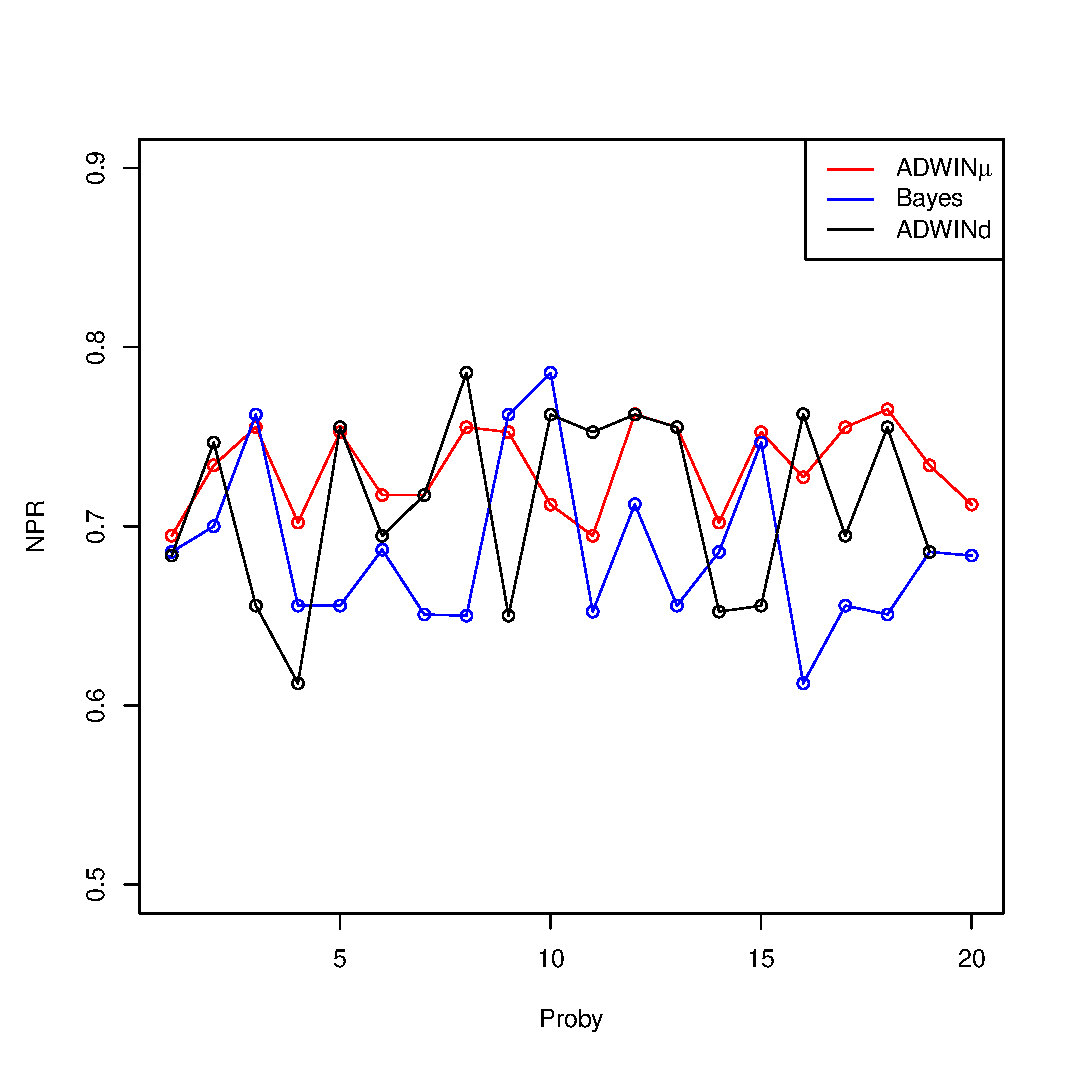
\includegraphics[width=0.6\textwidth]{img/ch-5-jump-res-npr}
  \caption{Wyniki dla poszczególnych prób -- współczynnik fałszywych alarmów}
  \label{fig:JumpingValuesResNpr}
\end{figure}

\newpage
Na wykresie \ref{fig:CovValues} przedstawiono przykładowy przebieg wartości dla pierwszych 5 zmian
wraz z zaznaczonymi miejscami,
gdzie nastąpiła.
\begin{figure}[htbp]
  \centering
  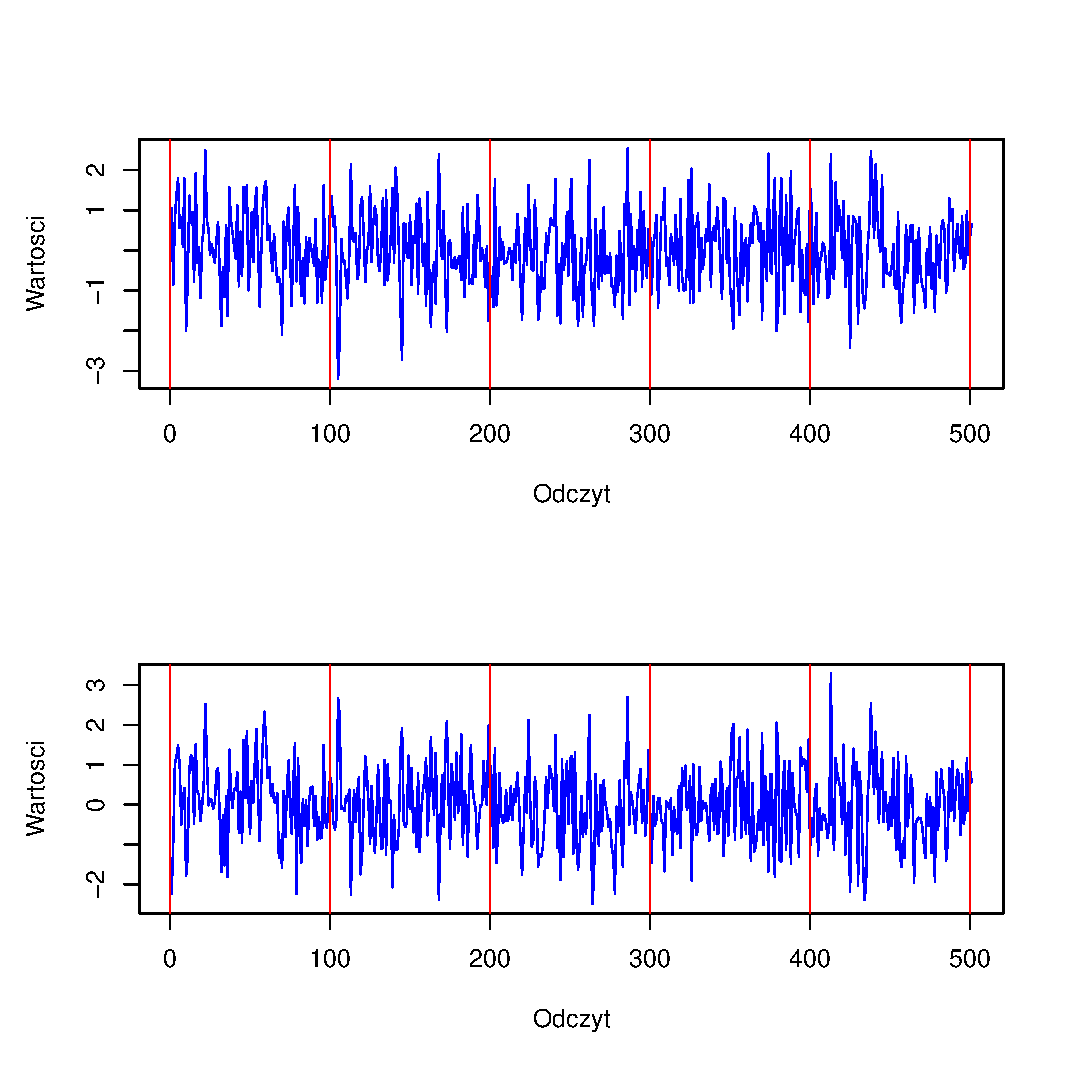
\includegraphics[width=0.8\textwidth]{img/ch-5-cov}
  \caption{Przykładowe wartości}
  \label{fig:CovValues}
\end{figure}
Na górnym rysunku przedstawiono pierwszy wymiar, na niższym drugi.
Badanie przeprowadzono poprzez wygenerowanie 20 zestawów danych.
Dla wszystkich zestawów w tabeli \ref{tab:JumpingResult} przedstawiono średnią oraz wariancje współczynników sukcesu i fałszywych alarmów.
\begin{table}[h]
  \label{tab:JumpingResult}
  \centering
  \begin{tabular}{l r r r r}
    & \multicolumn{2}{l}{TPR} & \multicolumn{2}{l}{NPR} \\
    \hline
    & \multicolumn{1}{l}{Średnia} & \multicolumn{1}{l}{Wariancja}& \multicolumn{1}{l}{Średnia} & \multicolumn{1}{l}{Wariancja} \\
    \hline
    BAY & do wstawienie & do wstawienia & do wstawienie & do wstawienia \\
    $ADW_{d}$ & do wstawienie & do wstawienia & do wstawienie & do wstawienia \\
  \end{tabular}
\end{table}

\subsection{Czujnik światła i zbliżeniowy}
Testom poddano dane zebrane przez czujnik natężenia światła oraz czujnik zbliżeniowy.
Jeśli ktoś je przesłonił wartości zmieniały się jednocześnie.
Dodatkowo na odczyty czujnika natężenia miała wpływ pora dnia (rys. \ref{fig:DeviceLightRes}).
Dane zostały zebrane z okresu trzech dni.
\begin{figure}[htbp]
  \centering
  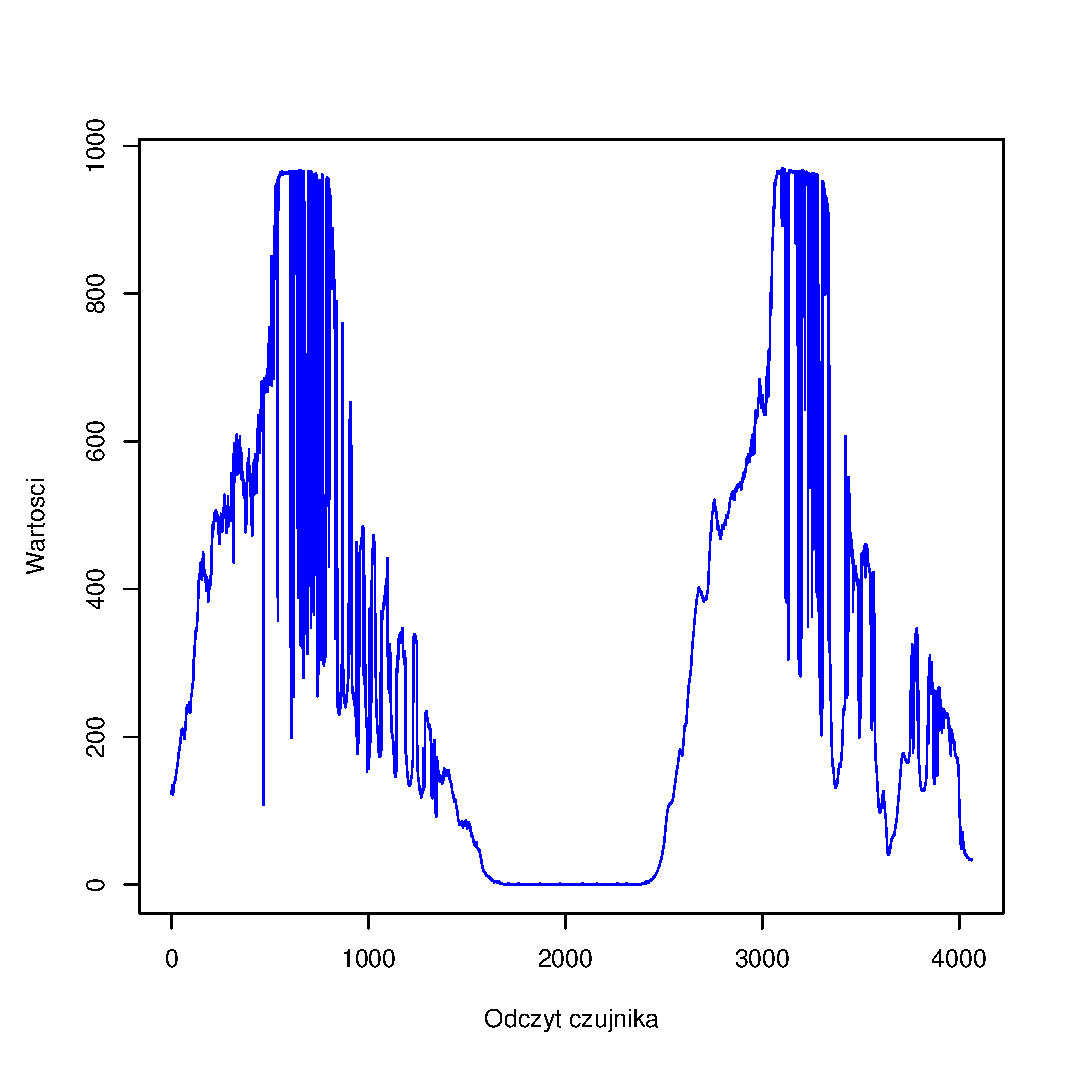
\includegraphics[width=0.6\textwidth]{img/ch-5-device-light}
  \caption{Odczyt czujnika światła -- dwa dni}
  \label{fig:DeviceLightRes}
\end{figure}

Zebrane dane analizowano jako dwa oddzielne strumienie jednowymiarowych próbek.
Jako poprawną zmianę przyjęto jako jednoczesne zasygnalizowanie zmian w obydwu badanych czujnikach.
Aby uznać zmianę za jednoczesną różnica czasowa pomiędzy próbkami może wynosić co najwyżej 20 próbek.

\subsubsection*{Czujnik światła}
Z uwagi na wrażliwość czujnika na porę dnia,
przekładającą się na wahania wartości algorytmy częściej powinny wykrywać zmiany.
Oczekiwania teoretyczne potwierdziły się -- tabela \ref{tab:LightResutl}.
Wszystkie algorytmy osiągneły zbliżony poziom, wykrywając zmianę średnio co 60 sekund.
\begin{table}[h]
  \label{tab:LightResutl}
  \centering
  \begin{tabular}{l r }
    Algorytm & \multicolumn{1}{l}{Liczba wykrytych zmian} \\
    \hline
    BAY & 4335  \\
    $\mbox{ADW}_{\mu}$ & 5050 \\
    $\mbox{ADW}_{d}$ & 4757  \\
  \end{tabular}
  \caption{Liczba wykrytych zmian -- czujnik światła}
\end{table}
\clearpage
\subsubsection*{Czujnik zbliżeniowy}
Charakterystyka tego czujnika jest bardziej stabilna.
Otrzymywane wartości ulegają zmianie, dopiero gdy coś się zbliża.
Widać to wyraźnie na otrzymanych wynikach (tabela \ref{tab:DistResutl}).
Liczba zaobserwowanych zmian jest mniejsza.
\begin{table}[h]
  \label{tab:DistResutl}
  \centering
  \begin{tabular}{l r }
    Algorytm & \multicolumn{1}{l}{Liczba wykrytych zmian} \\
    \hline
    BAY & 178 \\
    $\mbox{ADW}_{\mu}$ & 163 \\
    $\mbox{ADW}_{d}$ & 167\\
  \end{tabular}
  \caption{Liczba wykrytych zmian -- czujnik zbliżeniowy}
\end{table}

\subsubsection*{Wyniki sumaryczne}
Po skorelowaniu danych pojeńczych wyniki sumaryczne przedstawiono w tabeli \ref{tab:DevAllResutl}.
Niestety podobnie jak w przypadku testu skaczącej średniej algorytmy osiągnęły wysoki współczynnik fałszywych alarmów.
\begin{table}[h]
  \label{tab:DevAllResutl}
  \centering
  \begin{tabular}{l r}
    Algorytm & \multicolumn{1}{l}{Liczba wykrytych zmian} \\
    \hline
    BAY & 89 \\
    $\mbox{ADW}_{\mu}$ & 98 \\
    $\mbox{ADW}_{d}$ & 104 \\
  \end{tabular}
  \caption{Liczba wykrytych zmian -- wyniki sumaryczne}
\end{table}
Ponieważ analizowane dane pochodziły bezpośrednio z czujników,
nie były wcześniej przetwarzane,
to szum pomiarowy mógł mieć zauważalny wpływ na otrzymane wyniki.
Zastosowanie filtrów wygładzających przebiegi powinno obniżyć wskaźnik NPR.

\section{Podsumowanie}
Wyniki przeprowadzonych testów pokazują,
że możliwe jest wykorzystanie współczesnych platform do analizy strumieniowej
do problemu wykrywania zmian.
Wszystkie algorytmy z rozdziału \ref{ch:algo} osiągnęły skuteczność w wykrywaniu zmian
na poziomie około 30\% do 50\%.
Metody oparte o okno przesuwne (ADWIN) okazały się jednak skuteczniejsze.

W przypadku danych jednowymiarowych otrzymane wyniki dla rodziny ADWIN były bardzo do siebie zbliżone.
Rożnica pomiędzy nimi pojawiła się dopiero podczas testów na danych wielowymiarowych.
Z uwagi na budowę swojego testu $\mbox{ADWIN}_\mu$, opartego na średniej i wariancji,
nie był w stanie wykrywać zmian.
$\mbox{ADWIN}_d$ oparty na generycznych teście ilorazu gęstości rozkładu prawdopodobieństw radził sobie bez problemów.
Niestety obarczony był dużym narzutem wydajnościowym,
związanym z koniecznością rozwiązania zadania optymalizacyjnego podczas obliczania estymaty ilorazu.

Wszystkie badane algorytmy cechowały się dużym współczynnikiem generowanych fałszywych alarmów.
Najprawdopodobniej wynika to z braku wcześniejsze pre-procesowania danych wejściowych.
Jako pre-processing można rozumieć na przykład wygładzenie przebiegów poprzez użycie różnego rodzaju filtrów.

Przeprowadzone eksperymenty pokazują,
że nie ma algorytmu idealnego (uniwersalnego),
pasującego do wszystkich kategorii problemów.
Każdy z nich pasuje do innych sytuacji.
$\mbox{ADWIN}_\mu$ nie obsługuje danych wielowymiarowych,
ale za to skutecznie wykrywa zmiany w środowisku jednowymiarowym.
Dodatkowo charakteryzuje się małym zapotrzebowaniem na zasoby i bardzo szybkimi odpowiedziami.
$\mbox{ADWIN}_\mu$ efektywnie wykrywa zmiany w rozkładach jedno i wielowymiarowych,
jednak charakteryzuje się dużą złożonością i wysokimi czasami odpowiedzi,
co niestety nie pozwala na jego wykorzystanie praktyczne.
Algorytm Bayesa także wykrywa zmiany w rozkładach jedno i wielowymiarowych.
Jego mankamentem jest konieczność wcześniejszego znania rozkładu jakim opisane są próbki,
przez co nie można go zastosować do rozwiązywania generycznych problemów.

